\documentclass{article}
\usepackage{graphicx}
\usepackage{subcaption}
\usepackage[margin=1in]{geometry}
% Allows filenames with spaces
\usepackage[space]{grffile}

\begin{document}

\begin{figure}[htbp]
    \centering
    \textbf{Attention Layer 1} \\[0.5em]
    \begin{subfigure}[b]{0.45\textwidth}
        
\includegraphics[width=\textwidth]{"attention_2/Attention_only/attention/media/images/Attention 0_600_79db42d35371d577543e.png"}
        \caption{Time 600}
    \end{subfigure}
    \hfill
    \begin{subfigure}[b]{0.45\textwidth}
        
\includegraphics[width=\textwidth]{"attention_2/Attention_only/attention/media/images/Attention 0_1100_861f4ed65ff341408fad.png"}
        \caption{Time 1100}
    \end{subfigure}
    
    \vspace{0.5cm}
    \begin{subfigure}[b]{0.45\textwidth}
        
\includegraphics[width=\textwidth]{"attention_2/Attention_only/attention/media/images/Attention 0_1600_ac4e4f69b3067f348662.png"}
        \caption{Time 1600}
    \end{subfigure}
    \hfill
    \begin{subfigure}[b]{0.45\textwidth}
        
\includegraphics[width=\textwidth]{"attention_2/Attention_only/attention/media/images/Attention 0_2300_d1c37f6e82b4e969d760.png"}
        \caption{Time 2300}
    \end{subfigure}

    \vspace{1cm}

    \textbf{$Q^{\top}K$ Layer 2} \\[0.5em]
    \begin{subfigure}[b]{0.35\textwidth}
        
\includegraphics[width=\textwidth]{"attention_2/Attention_only/attention/media/images/A_2_600_c98abeb589af1e7fca07.png"}
        \caption{Time 600}
    \end{subfigure}
    \hspace{0.1\textwidth}
    \begin{subfigure}[b]{0.35\textwidth}
        
\includegraphics[width=\textwidth]{"attention_2/Attention_only/attention/media/images/A_2_1100_33682095ae2d3a1e3194.png"}
        \caption{Time 1100}
    \end{subfigure}
    
    \vspace{0.25cm}
    \begin{subfigure}[b]{0.35\textwidth}
        
\includegraphics[width=\textwidth]{"attention_2/Attention_only/attention/media/images/A_2_1600_55510a8f0380c13d0cfd.png"}
        \caption{Time 1600}
    \end{subfigure}
    \hspace{0.1\textwidth}
    \begin{subfigure}[b]{0.35\textwidth}
        
\includegraphics[width=\textwidth]{"attention_2/Attention_only/attention/media/images/A_2_2300_c8bc8463802da8c4f2c3.png"}
        \caption{Time 2300}
    \end{subfigure}

    \caption{\textbf{Q,K in second layer with random initialization.} Plots for $k=5$ and $l=120$ without assumption A1, A2. We use Gaussian initialization for $Q$ and $K$ with variance 0.1, making $Q^{\top}K$ random at initialization as is evident from time 600. We see the evolution of the second layer where the top principal diagonal of the block matrix aligns with $\tilde{I}$. Although other blocks also move, the main principal diagonal stays close to our simplification.}
    \label{fig:attention_comparison_times}
\end{figure}

\clearpage

\begin{figure}[htbp]
    \centering
    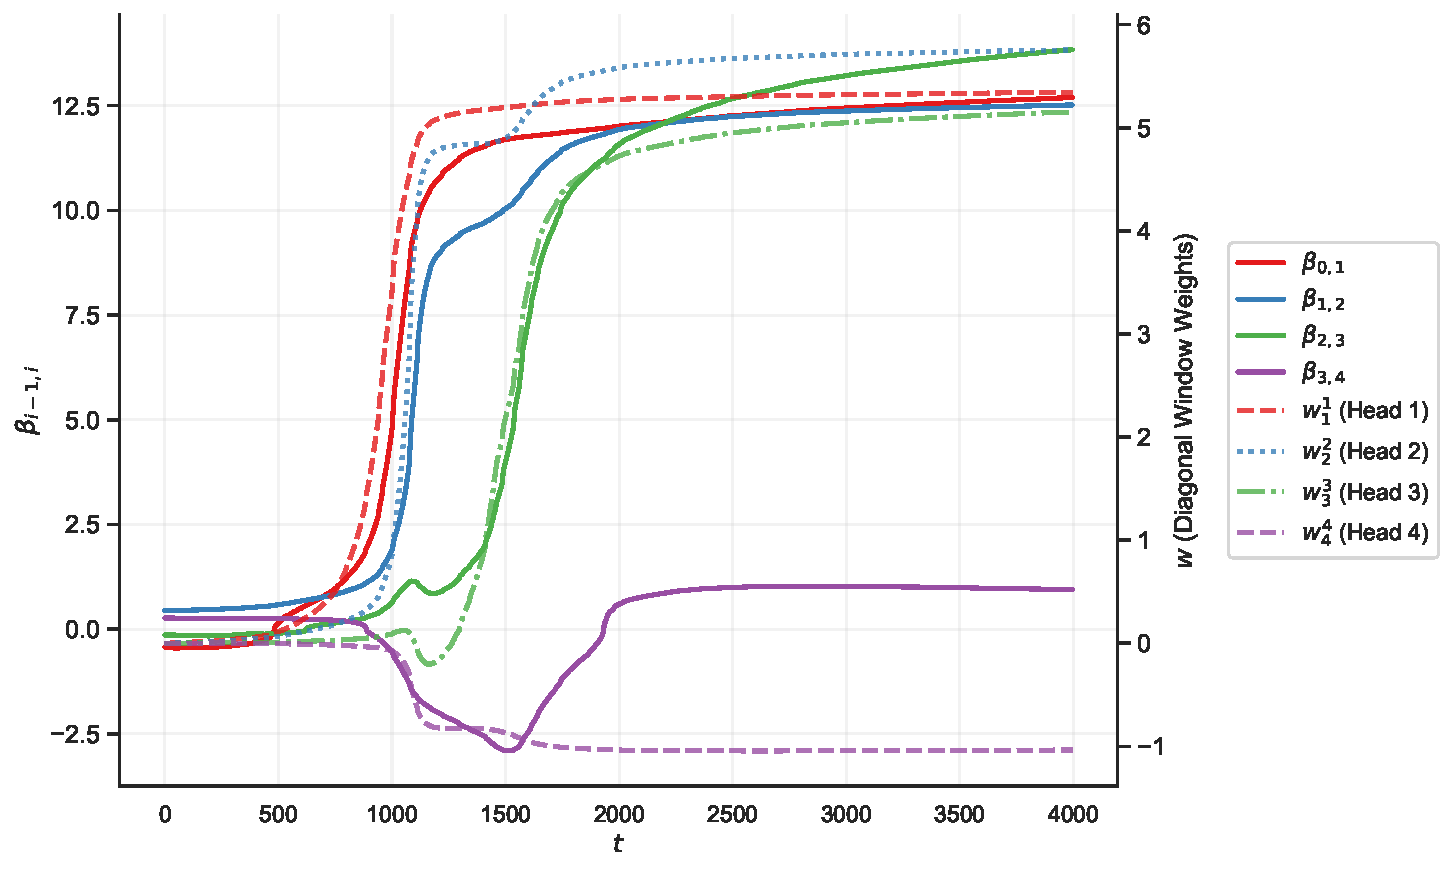
\includegraphics[width=\textwidth]{attention_2/xksepgn7_betas_window_combined.pdf}
    \caption{\textbf{Betas and Window Weights with full Q,K initialization.} Again for the same setting as Figure~\ref{fig:attention_comparison_times}. We plot the attention weights and also the betas. We compute the betas by taking the inner product of the blocks of $Q^{\top}K$ with $I$. We see that the betas, attention weights are tied and evolve in a way that is consistent with our conservative law and theory. The triaing is not complete as it is taking a long time to leave the last plateau.}
    \label{fig:xksepgn7_betas_window_combined}
\end{figure}

% \begin{figure}[htbp]
%     \centering
%     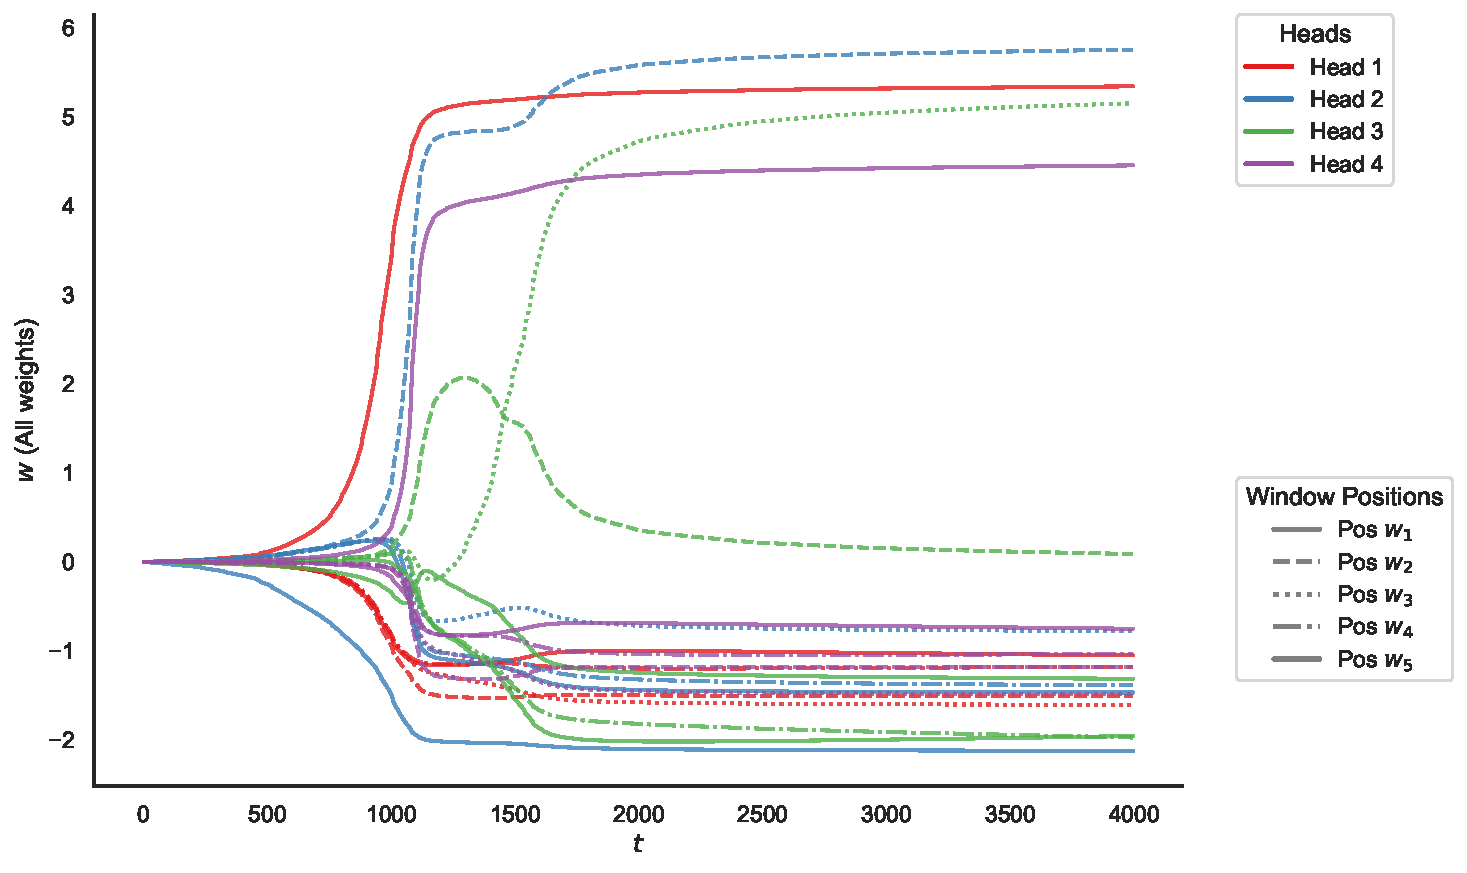
\includegraphics[width=\textwidth]{attention_2/xksepgn7_all_window_weights.pdf}
%     \caption{All window weights across time for run xksepgn7.}
%     \label{fig:xksepgn7_all_window_weights}
% \end{figure}

\begin{figure}[htbp]
    \centering
    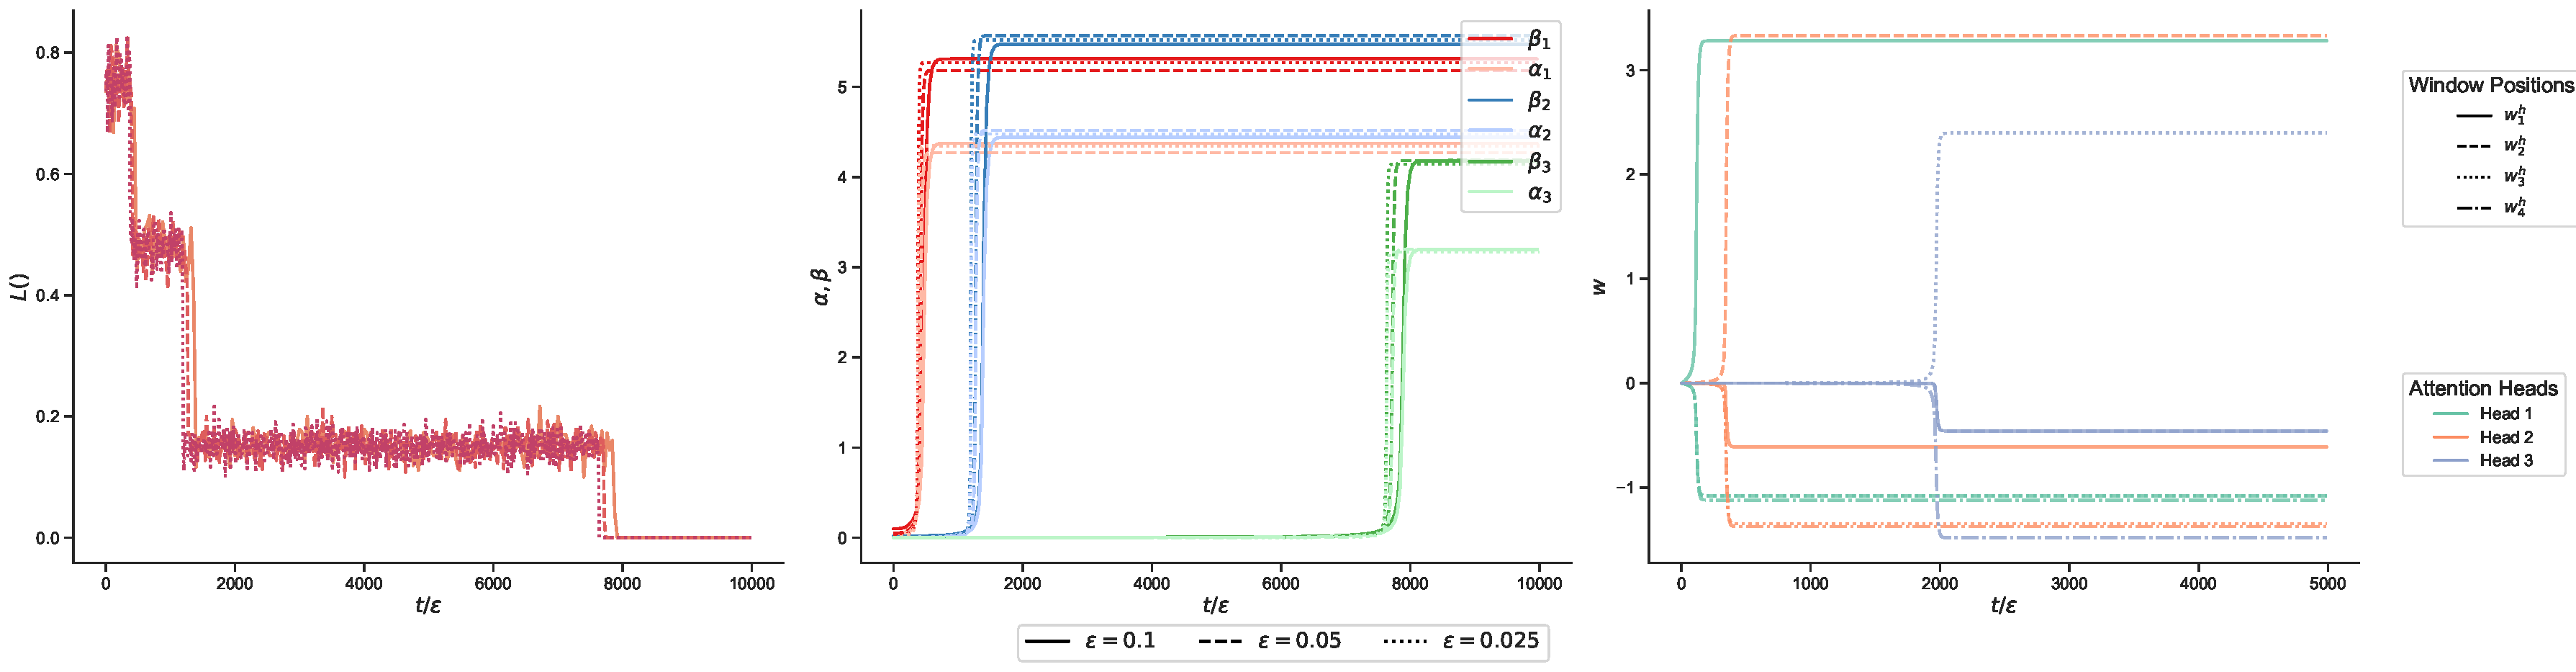
\includegraphics[width=\textwidth]{combined_plots.pdf}
    \caption{Incomplete permutations for $k=4$ and length = 60 at various scales trained with cross entropy and with assumptions A(0)-A(4). It validates the timescales and conservative law when all the permutations are not present in the context.}
    \label{fig:combined_plots}
\end{figure}

\end{document}
